% %% %%%%%%%%%%%%%%%%%%%%%%%%%%%%%%%%%%%%%%%%%%%%%%%%%%%%%%%%%%
% step-5.tex
%
% Author:  Mauricio Matamoros
% License: MIT
%
% %% %%%%%%%%%%%%%%%%%%%%%%%%%%%%%%%%%%%%%%%%%%%%%%%%%%%%%%%%%%

%!TEX root = ../main.tex
%!TEX root = ../references.bib

\subsection{Paso 5: Configuración de la Raspberry Pi como servidor Web}%
\label{sec:webserver}

Raspbian es una variante d Debian, por lo que se le dará bien servir páginas web de forma segura, especialmente cuando se utiliza Apache.
Sin embargo, configurar Apache para enlazarse con Python y operar la GPIO no es una tarea trivial, por lo que en esta práctica se utilizará un servidor web simple basado en el \texttt{BaseHTTPRequestHandler} que incorpora el paquete \texttt{http.server} de Python.

Para habilitar un servidor web en Python, basta con heredar de la clase \texttt{BaseHTTPRequestHandler} e implementar el método \texttt{do\_GET} para que imprima el código HTML al socket vía el método \texttt{self.wfile.write} tal como se muestra en el \Cref{lst:simple-webserver}.

\lstinputlisting[%
	firstline=17,
	lastline=35,
	label={lst:simple-webserver},
	caption=Archivo \texttt{simple-webserver.py}
]{src/simple-webserver.py}

Script de Python presentado inicia un servidor web que atiende todas las peticiones entrantes vía la interfaz con la IP 192.168.1.254 (el punto de acceso) en el puerto 80 (HTTP predeterminado).
A cada petición se le devolverá una señal de estado HTTP200 u \emph{OK}, seguido por código HTML. % CHKTEX 13
Es importante aclarar que para cada archivo servido se debe especificar el tipo de archivo en la cabecera.

\paragraph*{Importante:} El puerto 80 (y en general todos los puertos por debajo del 2014) están reservados para servicios de sistema, por lo que Python fallará al intentar levantar el servidor web en este puerto. Existen dos opciones: puede ejecutar el proceso como superusuario con \texttt{sudo} o bien usar otro puerto como el 8080.

Genere el archivo \texttt{simple-webserver.py} y ejecútelo.
A continuación, conéctese a la Raspberry Pi con cualquier dispositivo móvil e ingrese a la dirección IP del punto de acceso, es decir: \url{http://192.168.1.254}.

Con ligeras modificaciones es posible servir cualquier tipo de archivo.
Todas las peticiones ingresadas en la barra de direcciones del navegador llegarán por método \emph{GET}, por lo que deberán ser procesadas en el método \texttt{do\_GET}, accediendo al atributo de clase \texttt{self.path}, relativo al directorio de trabajo.
En caso de que no se proporcione un archivo, \texttt{do\_GET} tendrá que proporcionar la página por defecto, típicamente nombrada \texttt{index.html}, pero que en este caso por motivos didácticos se ha nombrado \texttt{user\_interface.html} (véase \Cref{lst:webserver-get}).

\lstinputlisting[%
	firstline=79,
	lastline=96,
	label={lst:webserver-get},
	caption=Método \texttt{do\_GET} del archivo webserver.py
]{src/webserver.py}

Para servir un archivo se tiene que verificar que el éste exista, proporcionar su tipo mime en la cabecera y devolver los datos como una cadena binaria.
Esto se realiza en el método interno \texttt{\_serve\_file}.
Si el archivo no se encontrare, se devuelve un error \emph{HTTP404} como se muestra en el \Cref{lst:webserver-serve}:

\lstinputlisting[%
	firstline=36,
	lastline=45,
	label={lst:webserver-serve},
	caption=Método \texttt{\_serve\_file} del archivo webserver.py
]{src/webserver.py}

La interacción cliente servidor se lleva a cabo de manera similar.
Dependerá de si los datos se envían por método \emph{GET} o \emph{POST}, de los cuales se prefiere el segundo pues hace más difícil inyectar datos.
De manera análoga se utiliza el método \texttt{do\_POST} que recibe y procesa los datos.
En esta práctica, se utilizan dados codificados mediante JSON para hacer llamadas asíncronas del cliente y sin respuesta por parte del servidor (véase \Cref{lst:webserver-post}).

\lstinputlisting[%
	firstline=103,
	lastline=117,
	label={lst:webserver-post},
	caption=Método \texttt{do\_POST} del archivo webserver.py
]{src/webserver.py}

El método \texttt{do\_POST} preentado en el \Cref{lst:webserver-post} interpreta los datos recibidos como cadenas de texto unicode de 8 bits (\emph{utf-8}) que contienen objetos en JSON que son decodificados a un diccionario de Python.
El diccionario es después enviado al método interno \texttt{\_parse\_post} mostrado en el \Cref{lst:webserver-parse-post} que analiza los datos y realiza las acciones pertinentes.

\lstinputlisting[%
	firstline=62,
	lastline=73,
	label={lst:webserver-parse-post},
	caption=Método \texttt{\_parse\_post} del archivo webserver.py
]{src/webserver.py}

Genere los archivos \texttt{webserver.py} y \texttt{user\_interface.html} (véase \Cref{sec:webserver-py,sec:ui-html}), luego ejecute el scrypt de Python.
A continuación, conéctese a la Raspberry Pi con cualquier dispositivo móvil e ingrese a la dirección IP del punto de acceso, es decir: \url{http://192.168.1.254}.
Debería ver una pantalla similar a la siguiente.

\begin{figure}[H]
	\centering
	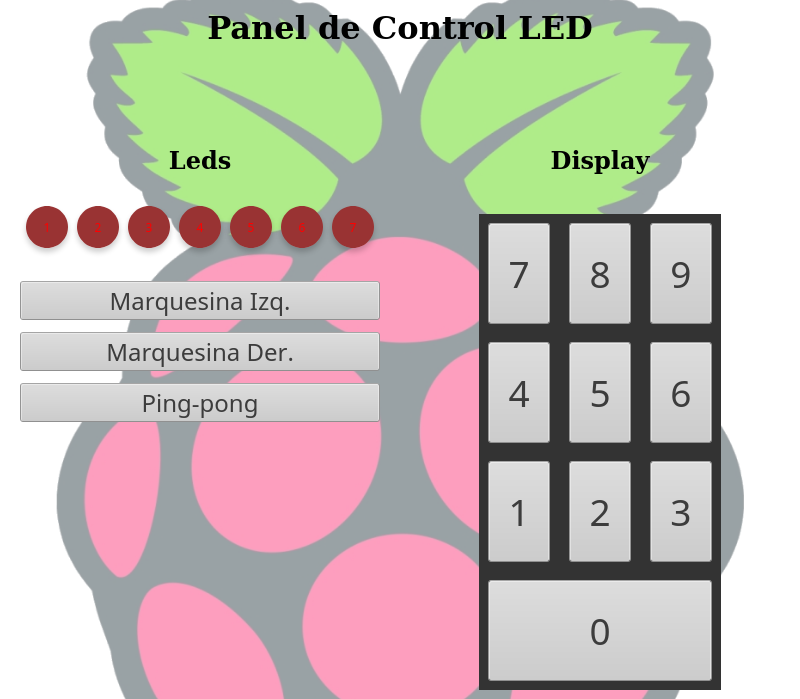
\includegraphics[height=7cm,keepaspectratio]{img/screenshot-ui.png}
	\caption{Caption: Intefaz de usuario del controlador de Leds en la Raspberry Pi.}
	\label{fig:hello-world} %CHKTEX 24
\end{figure}


